\documentclass[twoside,bind,paper=a4,ams,booktabs]{hepthesis}
%\documentclass[twoside,bind,draft,paper=a4,ams,booktabs]{hepthesis}


%% Load special font packages
%\usepackage{mathpazo}    %palotino?   %Screws up Gauge link variables U appearance slightly

%%Package includes, custom commands in preamble
%%Use this file for package inclusion or defined commands
%\usepackage{float}             %for using [H] option in figures to fix position
\usepackage{placeins}
\usepackage{changepage}
\usepackage{graphicx}          %for importing pictures
\usepackage{slashed}           %for Feynman slash notation
\usepackage{braket}            %for bra-ket notation
\usepackage{color}             %for \textcolor
\usepackage{cite}              %To get [3-5] instead of [3,4,5]
\usepackage{hepunits}          %Consistent units
\usepackage{amssymb}           %For upharpoonleft, etc
\usepackage{dsfont}            %For double line 1
\usepackage{simplewick}        %For wick contractions
\usepackage{subcaption}        %Subfigures
\usepackage{adjustbox}         %For making the chiEFT coeffs table fit better
\usepackage{multicol}
\usepackage{tikz}
\usepackage{pgfplots}
\usepackage{tikz-feynman}
\usepackage{lineno}
\usepackage[utf8]{inputenc}    %For nice characters in a couple of references
\linenumbers
\definecolor{tab10Green}{rgb}{0.1726,0.6275,0.1726}
\definecolor{tab10Red}{rgb}{0.8392,0.1530,0.1569}
\definecolor{tab10Blue}{rgb}{0.1216,0.4667,0.7059}
\DeclareSIUnit\barn{b}
\usetikzlibrary{arrows.meta,bending,positioning}
%%Doc-Specific PDF metadata
\setcounter{secnumdepth}{4}% for subsubsection numbering 
\usepackage[%
        pdfusetitle,
        pdfsubject={PhD thesis},
        pdfkeywords={YOUR FAVE KEYWORDS,HEP,particle,Belle II,Physics,thesis},
        colorlinks=true,         %color the links, not boxes
        citecolor=tab10Green,    %Change colors of citations
        linkcolor=black,         %All internal links. contents page, etc %Eqn/fig set in main.tex hypersetup
        %filecolor=blue,         %Unsure
        %anchorcolor=green,      %Unsure
        %menucolor=red,          %Unsure
        urlcolor=tab10Blue,      %Color of URLs in bib
        backref=section]{hyperref}

%Making the square brackets on a cite also the citecolor (manually). Does not make them hyperlinks
%\renewcommand{\citeleft}{\textcolor{tab10Green}{[}}
%\renewcommand{\citeright}{\textcolor{tab10Green}{]}}

%For Drafting purposes
\newcommand{\tcr}[1]{\textcolor{magenta}{#1}}
%Bracketing commands
\newcommand{\rb}[1]{\left(#1\right)}
\DeclareRobustCommand{\sq}[1]{\left[#1\right]}
%one sided round brackets
\newcommand{\bre}[1]{\left(#1\right.}
\newcommand{\ebr}[1]{\left.#1\right)}
%No sided brackets
\newcommand{\eeb}[1]{\left.#1\right.}
%One sided square brackets
\newcommand{\sqe}[1]{\left[#1\right.}
\newcommand{\esq}[1]{\left.#1\right]}
\newcommand{\acom}[2]{\left\{#1,\,#2\right\}}


\DeclareRobustCommand{\eqnr}[1]{Eq.~$\left(\ref{#1}\right)$}
\newcommand{\eqnrtwo}[2]{Eqs.~$\rb{\ref{#1}}$ and $\rb{\ref{#2}}$}
\newcommand{\eqnrthree}[3]{Eqs.~$\rb{\ref{#1}}$,$\rb{\ref{#2}}$ and $\rb{\ref{#3}}$}
\newcommand{\Fig}[1]{Figure \ref{#1}}
\newcommand{\Tab}[1]{Table \ref{#1}}
\newcommand{\Sec}[1]{Section \ref{#1}}
\newcommand{\Figtwo}[2]{Figures \ref{#1} and \ref{#2}}
\newcommand{\Figthree}[3]{Figures \ref{#1}, \ref{#2} and \ref{#3}}
\newcommand{\Chap}[1]{Chapter \ref{#1}}
\newcommand{\Chaptwo}[2]{Chapters \ref{#1} and \ref{#2}}
\newcommand{\App}[1]{Appendix \ref{#1}}

\newcommand{\Refl}[1]{Ref.~\cite{#1}}    %Might need to make more often than usual
\newcommand{\Refltwo}[2]{Refs.~\cite{#1} and \cite{#2}}    %Might need to make more often than usual


%Commands which are in physics.sty which I won't be using cause it screws up compiler error checking
\DeclareRobustCommand{\order}[1]{\mathcal{O}\left(#1\right)}
%absolute value
\DeclareRobustCommand{\abs}[1]{\left\lvert #1 \right\rvert }

% Easily switch  between arrow notation (standard) and bold (uncommented) notation for 3-vectors
%\let\oldvec\vec
%\renewcommand{\vec}[1]{\boldsymbol{#1}}

% Belle II def aliases
%%%%%   Standard symbols for use in Belle II notes and papers. 
%%%%%
%%%%%	C. Hearty	21-Oct-2014		Based on babarsym.tex; authored by D. Hitlin, D. MacFarlane, P. Dauncey, and R. Waldi
%%%%%

\RequirePackage{xspace}
\def\datafb {\qty{362}{\femto\barn^{-1}}}
%%%%%%%%%%%%sadlm edits
\def\BDpi {\ensuremath{B^{+}\to\bar{D}^{0}\pi^{+}}\xspace}
\def\sqrts {\ensuremath{\sqrt{s}}\xspace}
\def\DDbar {\ensuremath{D\bar{D}}\xspace}
\def\Vub {\ensuremath{V_{ub}}}
\def\fB {\ensuremath{f_{B}}\xspace}
\def\Bmunu {\ensuremath{\Bp\to\mup\num}\xspace}
\def\plep   {\ensuremath{p^{*}_{\ell}}\xspace}
\def\cmsp   {\ensuremath{p^{*}_{\mu}}\xspace}
\def\cmsppi   {\ensuremath{p^{*}_{\pi}}\xspace}
\def\Mx  {\ensuremath{M_X}\xspace}
\def\Bmtag   {\ensuremath{\Bm_{\text{tag}}}\xspace}
\def\Bmtags   {\ensuremath{\Bm_{\text{tag}}\'s}\xspace}
\def\Bptag   {\ensuremath{\Bp_{\text{tag}}}\xspace}
\def\Bptag   {\ensuremath{\Bm_{\text{tag}}}\xspace}
\def\Bptags   {\ensuremath{\Bp_{\text{tag}}\'s}\xspace}
\def\Btag   {\ensuremath{B_{\text{tag}}}\xspace}
\def\Btags   {\ensuremath{B_{\text{tag}}\'s}\xspace}
\def\Bsig   {\ensuremath{B_{\text{sig}}}\xspace}
\def\Bpsig   {\ensuremath{\Bp_{\text{sig}}}\xspace}
\def\Bmsig   {\ensuremath{\Bm_{\text{sig}}}\xspace}
\def\Btagell {\ensuremath{B_{\text{tag}}\ell}\xspace}
\def\SSB {\ensuremath{\frac{S}{\sqrt{S+B}}}\xspace}
\def\ssb {\ensuremath{\frac{S}{\sqrt{S+B}}}\xspace}
\def\epemBB {\ensuremath{e^{+}e^{-}\to B\bar{B}}\xspace}
\def\logtensigProb {\ensuremath{\mathrm{log}_{10}(\sigProb)}\xspace}
\def\sigProb {\texttt{sigProb}\xspace}
\def\basftwo {\texttt{basf2}\xspace}
\def\iSnu {\texttt{isSignalAcceptMissingNeutrino}\xspace}
\def\Ecms {\ensuremath{E_{\text{CMS}}}\xspace}
%\def\Vcb {\ensuremath{\|V_{cb}\|\xspace}
\def\Mbc {\ensuremath{M_{\text{bc}}}\xspace}
\def\deltaE {\ensuremath{\Delta E}\xspace}
\def\musig {\ensuremath{\mu_{\text{sig}}}\xspace}
\def\elltag {\ensuremath{\ell_{\text{tag}}}\xspace}
\def\mutag {\ensuremath{\mu_{\text{tag}}}\xspace}
\def\roeEextra {\ensuremath{E_{\text{ECL}}}}
\def\BF {\ensuremath{\mathcal{B}(\Bmunu)}\xspace}
%\def\CMSp#1 {\ensuremath{\vec{p}_{#1}^{\kern 0.16em *}}\xspace} 
%\def\Y#1S{\ensuremath{\Upsilon{(#1S)}}\xspace}% no space before {...}!
%%%%%%%%%%%%%%%%%%%% THE NAME OF THE COLLABORATION %%%%
\def\belletwo {Belle~II~}
\def\cosThetaBY {\ensuremath{\mathrm{cos}\,\theta_{BY}}\xspace}
\def\cosTBTO {\ensuremath{\mathrm{cos}\,\theta_{T_{B}T_{\text{ROE}}}}\xspace}
\def\thetaBY {\ensuremath{\theta_{BY}}\xspace}
\def\mathcalB {\ensuremath{\mathcal{B}}}
\def\cosThetapmiss {\ensuremath{\mathrm{cos}\,\theta_{\overrightarrow{p}_{\text{miss}}}}}


%%%%%%%%%%%%%%%%%%%%%%%%%%%%%%%%%%%%%%%%%%%%%%%
%%%%%%%%%%%%%%%%%   LEPTONS   %%%%%%%%%%%%%%%%%
%%%%%%%%%%%%%%%%%%%%%%%%%%%%%%%%%%%%%%%%%%%%%%%
\let\emi\en
\def\electron   {\ensuremath{e}\xspace}
\def\en         {\ensuremath{e^-}\xspace}   % electron negative (\em is taken)
\def\ep         {\ensuremath{e^+}\xspace}
\def\epm        {\ensuremath{e^\pm}\xspace} 
\def\epem       {\ensuremath{e^+e^-}\xspace}
\def\ee         {\ensuremath{e^-e^-}\xspace}

\def\mmu        {\ensuremath{\mu}\xspace}
\def\mup        {\ensuremath{\mu^+}\xspace}
\def\mun        {\ensuremath{\mu^-}\xspace} % muon negative (\mum is taken)
\def\mumu       {\ensuremath{\mu^+\mu^-}\xspace}
\def\mtau       {\ensuremath{\tau}\xspace}

\def\taup       {\ensuremath{\tau^+}\xspace}
\def\taum       {\ensuremath{\tau^-}\xspace}
\def\tautau     {\ensuremath{\tau^+\tau^-}\xspace}

\def\ellm       {\ensuremath{\ell^-}\xspace}
\def\ellp       {\ensuremath{\ell^+}\xspace}
\def\ellell     {\ensuremath{\ell^+ \ell^-}\xspace}

\def\nub        {\ensuremath{\overline{\nu}}\xspace}
\def\nunub      {\ensuremath{\nu{\overline{\nu}}}\xspace}
\def\nub        {\ensuremath{\overline{\nu}}\xspace}
\def\nunub      {\ensuremath{\nu{\overline{\nu}}}\xspace}
\def\nue        {\ensuremath{\nu_e}\xspace}
\def\nueb       {\ensuremath{\nub_e}\xspace}
\def\nuenueb    {\ensuremath{\nue\nueb}\xspace}
\def\num        {\ensuremath{\nu_\mu}\xspace}
\def\numb       {\ensuremath{\nub_\mu}\xspace}
\def\numnumb    {\ensuremath{\num\numb}\xspace}
\def\nut        {\ensuremath{\nu_\tau}\xspace}
\def\nutb       {\ensuremath{\nub_\tau}\xspace}
\def\nutnutb    {\ensuremath{\nut\nutb}\xspace}
\def\nul        {\ensuremath{\nu_\ell}\xspace}
\def\nulb       {\ensuremath{\nub_\ell}\xspace}
\def\nulnulb    {\ensuremath{\nul\nulb}\xspace}

%%%%%%%%%%%%%%%%%%%%%%%%%%%%%%%%%%%%%%%%%%%%%%%%%%
%%%%%%%%%%%%%%%%%%  PHOTONS  %%%%%%%%%%%%%%%%%%%%%
%%%%%%%%%%%%%%%%%%%%%%%%%%%%%%%%%%%%%%%%%%%%%%%%%%

\def\g     {\ensuremath{\gamma}\xspace}
\def\gaga  {\ensuremath{\gamma\gamma}\xspace}  %% changed from \gg, which is >>
\def\ggstar{\ensuremath{\gamma\gamma^*}\xspace}

\def\ega    {\ensuremath{e\gamma}\xspace}
\def\game   {\ensuremath{\gamma e^-}\xspace}
\def\epemg  {\ensuremath{e^+e^-\gamma}\xspace}

%%%%%%%%%%%%%%%%%%%%%%%%%%%%%%%%%%%%%%%%
%%%%  Other GAUGE BOSONS  %%%%%%%%%%%%%%
%%%%%%%%%%%%%%%%%%%%%%%%%%%%%%%%%%%%%%%%

\def\H      {\ensuremath{H^0}\xspace}
\def\Hp     {\ensuremath{H^+}\xspace}
\def\Hm     {\ensuremath{H^-}\xspace}
\def\Hpm    {\ensuremath{H^\pm}\xspace}
\def\W      {\ensuremath{W}\xspace}
\def\Wp     {\ensuremath{W^+}\xspace}
\def\Wm     {\ensuremath{W^-}\xspace}
\def\Wpm    {\ensuremath{W^\pm}\xspace}
\def\Z      {\ensuremath{Z^0}\xspace}

%%%%%%%%%%%%%%%%%%%%%%%%%%%%%%%%%%%%%%%%%%%%%%%%%%
%%%%%%%%%%%%%%%%%%   QUARKS   %%%%%%%%%%%%%%%%%%%%
%%%%%%%%%%%%%%%%%%%%%%%%%%%%%%%%%%%%%%%%%%%%%%%%%%

\def\q     {\ensuremath{q}\xspace}
\def\qbar  {\ensuremath{\overline q}\xspace}
\def\qqbar {\ensuremath{q\overline q}\xspace}
\def\u     {\ensuremath{u}\xspace}
\def\ubar  {\ensuremath{\overline u}\xspace}
\def\uubar {\ensuremath{u\overline u}\xspace}
\def\d     {\ensuremath{d}\xspace}
\def\dbar  {\ensuremath{\overline d}\xspace}
\def\ddbar {\ensuremath{d\overline d}\xspace}
\def\s     {\ensuremath{s}\xspace}
\def\sbar  {\ensuremath{\overline s}\xspace}
\def\ssbar {\ensuremath{s\overline s}\xspace}
\def\c     {\ensuremath{c}\xspace}
\def\cbar  {\ensuremath{\overline c}\xspace}
\def\ccbar {\ensuremath{c\overline c}\xspace}
\def\b     {\ensuremath{b}\xspace}
\def\bbar  {\ensuremath{\overline b}\xspace}
\def\bbbar {\ensuremath{b\overline b}\xspace}
\def\t     {\ensuremath{t}\xspace}
\def\tbar  {\ensuremath{\overline t}\xspace}
\def\tbar  {\ensuremath{\overline t}\xspace}
\def\ttbar {\ensuremath{t\overline t}\xspace}


%%%%%%%%%%%%%%%%%%%%%%%%%%%%%%%%%%%%%%%%%%%%%%%%%%
%%%%%%%%%%%%%%%%%% LIGHT MESONS  %%%%%%%%%%%%%%%%%
%%%%%%%%%%%%%%%%%%%%%%%%%%%%%%%%%%%%%%%%%%%%%%%%%%

\def\piz   {\ensuremath{\pi^0}\xspace}
\def\pizs  {\ensuremath{\pi^0\mbox\,\textrm{s}}\xspace}
\def\ppz   {\ensuremath{\pi^0\pi^0}\xspace}
\def\pip   {\ensuremath{\pi^+}\xspace}
\def\pim   {\ensuremath{\pi^-}\xspace}
\def\pipi  {\ensuremath{\pi^+\pi^-}\xspace}
\def\pipm  {\ensuremath{\pi^\pm}\xspace}
\def\pimp  {\ensuremath{\pi^\mp}\xspace}
\def\rhom  {\ensuremath{\rho^{-}}\xspace}
\def\rhop  {\ensuremath{\rho^{+}}\xspace}
\def\rhoz  {\ensuremath{\rho^{+}}\xspace}

\def\kaon  {\ensuremath{K}\xspace}
\def\K     {\ensuremath{K}\xspace}
%%% do NOT use ensuremath here
\def\Kbar  {\kern 0.2em\overline{\kern -0.2em K}{}\xspace}
\def\Kb    {\ensuremath{\Kbar}\xspace}
\def\Kz    {\ensuremath{K^0}\xspace}
\def\Kzb   {\ensuremath{\Kbar^0}\xspace}
\def\KzKzb {\ensuremath{\Kz \kern -0.16em \Kzb}\xspace}
\def\Kp    {\ensuremath{K^+}\xspace}
\def\Km    {\ensuremath{K^-}\xspace}
\def\Kpm   {\ensuremath{K^\pm}\xspace}
\def\Kmp   {\ensuremath{K^\mp}\xspace}
\def\KpKm  {\ensuremath{\Kp \kern -0.16em \Km}\xspace}
\def\Ks   {\KS} 
\def\KS    {\ensuremath{K^0_{\scriptscriptstyle S}}\xspace} 
\def\KL    {\ensuremath{K^0_{\scriptscriptstyle L}}\xspace} 
\def\Kstarz  {\ensuremath{K^{*0}}\xspace}
\def\Kstarzb {\ensuremath{\Kbar^{*0}}\xspace}
\def\Kstar   {\ensuremath{K^*}\xspace}
\def\Kstarb  {\ensuremath{\Kbar^*}\xspace}
\def\Kstarp  {\ensuremath{K^{*+}}\xspace}
\def\Kstarm  {\ensuremath{K^{*-}}\xspace}
\def\Kstarpm {\ensuremath{K^{*\pm}}\xspace}
\def\Kstarmp {\ensuremath{K^{*\mp}}\xspace}

\newcommand{\etapr}{\ensuremath{\eta^{\prime}}\xspace}


%%%%%%%%%%%%%%%%%%%%%%%%%%%%%%%%%%%%%%%%%%%%%%%%%%
%%%%%%%%%%%%%%%%%% HEAVY MESONS  %%%%%%%%%%%%%%%%%
%%%%%%%%%%%%%%%%%%%%%%%%%%%%%%%%%%%%%%%%%%%%%%%%%%

\def\D       {\ensuremath{D}\xspace}
%%% do NOT use ensuremath here
%\def\Dbar    {\kern 0.2em\overline{\kern -0.2em D}{}\xspace}
%\def\Bbar    {\kern 0.18em\overline{\kern -0.18em B}{}\xspace}
\def\Dbar    {\kern 0.2em\overline{\kern -0.2em D}{}\xspace}
\def\Db      {\ensuremath{\Dbar}\xspace}
\def\Dz      {\ensuremath{D^0}\xspace}
\def\Dzbar   {\ensuremath{\Dzb}}
\def\Dzb     {\ensuremath{\Dbar^0}\xspace}
\def\DzDzb   {\ensuremath{\Dz {\kern -0.16em \Dzb}}\xspace}
\def\Dp      {\ensuremath{D^+}\xspace}
\def\Dm      {\ensuremath{D^-}\xspace}
\def\Dpm     {\ensuremath{D^\pm}\xspace}
\def\Dmp     {\ensuremath{D^\mp}\xspace}
\def\DpDm    {\ensuremath{\Dp {\kern -0.16em \Dm}}\xspace}
\def\Dstar   {\ensuremath{D^*}\xspace}
\def\Dst     {\Dstar}
\def\Dstarb  {\ensuremath{\Dbar^*}\xspace}
\def\Dstarz  {\ensuremath{D^{*0}}\xspace}
\def\Dstarzb {\ensuremath{\Dbar^{*0}}\xspace}
\def\Dstarp  {\ensuremath{D^{*+}}\xspace}
\def\Dstarm  {\ensuremath{D^{*-}}\xspace}
\def\Dstarpm {\ensuremath{D^{*\pm}}\xspace}
\def\Dstarmp {\ensuremath{D^{*\mp}}\xspace}
\def\Ds      {\ensuremath{D^+_s}\xspace}
\def\Dsb     {\ensuremath{\Dbar^+_s}\xspace}
\def\Dss     {\ensuremath{D^{*+}_s}\xspace}


\def\B       {\ensuremath{B}\xspace}
%%% do NOT use ensuremath here
\def\Bbar    {\kern 0.18em\overline{\kern -0.18em B}{}\xspace}
\def\Bb      {\ensuremath{\Bbar}\xspace}
\def\BBbar      {\ensuremath{B\Bbar}\xspace} 
\def\BB      {\ensuremath{B\Bbar}\xspace} 
\def\Bz      {\ensuremath{B^0}\xspace}
\def\Bzb     {\ensuremath{\Bbar^0}\xspace}
\def\BzBzb   {\ensuremath{\Bz {\kern -0.16em \Bzb}}\xspace}
\def\Bu      {\ensuremath{B^+}\xspace}
\def\Bub     {\ensuremath{B^-}\xspace}
\def\Bp      {\ensuremath{\Bu}\xspace}
\def\Bm      {\ensuremath{\Bub}\xspace}
\def\Bpm     {\ensuremath{B^\pm}\xspace}
\def\Bmp     {\ensuremath{B^\mp}\xspace}
\def\BpBm    {\ensuremath{\Bu {\kern -0.16em \Bub}}\xspace}
\def\Bs      {\ensuremath{B_s}\xspace}
\def\Bsb     {\ensuremath{\Bbar_s}\xspace}
\def\BsBsb   {\ensuremath{$B_{s}\overline{B}_{s}$}\xspace}   
\def\BstBstb {\ensuremath{$B^{*}\overline{B}^{*}}\xspace}


%%%%%%%%%%%%%%%%%%%%%%%%%%%%%%%%%%%%%%%%%%%%%%%%%%
%%%%%%%%%%%%%%%%%%%%% ONIA %%%%%%%%%%%%%%%%%%%%%%%
%%%%%%%%%%%%%%%%%%%%%%%%%%%%%%%%%%%%%%%%%%%%%%%%%%

\def\jpsi     {\ensuremath{{J\mskip -3mu/\mskip -2mu\psi\mskip 2mu}}\xspace}
\def\Jpsi {\jpsi}
\def\psitwos  {\ensuremath{\psi{(2S)}}\xspace}
\def\psiprpr  {\ensuremath{\psi(3770)}\xspace}
\def\etac     {\ensuremath{\eta_c}\xspace}
\def\chiczero {\ensuremath{\chi_{c0}}\xspace}
\def\chicone  {\ensuremath{\chi_{c1}}\xspace}
\def\chictwo  {\ensuremath{\chi_{c2}}\xspace}
\mathchardef\Upsilon="7107
\def\Y#1S{\ensuremath{\Upsilon{(#1S)}}\xspace}% no space before {...}!
\def\OneS  {\Y1S}
\def\TwoS  {\Y2S}
\def\ThreeS{\Y3S}
\def\FourS {\Y4S}
\def\FiveS {\Y5S}
\def\SixS  {\Y6S}

\def\chic#1{\ensuremath{\chi_{c#1}}\xspace} 


%%%%%%%%%%%%%%%%%%%%%%%%%%%%%%%%%%%%%%%%%%%%%%%%%%
%%%%%%%%%%%%%%%%%%% BARYONS %%%%%%%%%%%%%%%%%%%%%%
%%%%%%%%%%%%%%%%%%%%%%%%%%%%%%%%%%%%%%%%%%%%%%%%%%

\def\proton      {\ensuremath{p}\xspace}
\def\antiproton  {\ensuremath{\overline p}\xspace}
\def\neutron     {\ensuremath{n}\xspace}
\def\antineutron {\ensuremath{\overline n}\xspace}

\mathchardef\Deltares="7101
\mathchardef\Xi="7104
\mathchardef\Lambda="7103
\mathchardef\Sigma="7106
\mathchardef\Omega="710A

%%% do NOT use ensuremath here
\def\Deltabar{\kern 0.25em\overline{\kern -0.25em \Deltares}{}\xspace}
\def\Lbar{\kern 0.2em\overline{\kern -0.2em\Lambda\kern 0.05em}\kern-0.05em{}\xspace}
\def\Sigbar{\kern 0.2em\overline{\kern -0.2em \Sigma}{}\xspace}
\def\Xibar{\kern 0.2em\overline{\kern -0.2em \Xi}{}\xspace}
\def\Obar{\kern 0.2em\overline{\kern -0.2em \Omega}{}\xspace}
\def\Nbar{\kern 0.2em\overline{\kern -0.2em N}{}\xspace}
\def\Xb{\kern 0.2em\overline{\kern -0.2em X}{}\xspace}

\def\X {\ensuremath{X}\xspace}


%%%%%%%%%%%%%%%%%%%%%%%%%%%%%%%%%%%%%%%%%%%%%%%%%%
%%%%%%%%%%%% ENERGY AND MOMENTUM %%%%%%%%%%%%%%%%%
%%%%%%%%%%%%%%%%%%%%%%%%%%%%%%%%%%%%%%%%%%%%%%%%%%

\newcommand{\tev}{\ensuremath{\mathrm{\,Te\kern -0.1em V}}\xspace}
\newcommand{\gev}{\ensuremath{\mathrm{\,Ge\kern -0.1em V}}\xspace}
\newcommand{\invgev}{\ensuremath{\mathrm{\,Ge\kern -0.1em V^{-1}}}\xspace}
\newcommand{\mev}{\ensuremath{\mathrm{\,Me\kern -0.1em V}}\xspace}
\newcommand{\kev}{\ensuremath{\mathrm{\,ke\kern -0.1em V}}\xspace}
\newcommand{\ev}{\ensuremath{\mathrm{\,e\kern -0.1em V}}\xspace}
\newcommand{\gevc}{\ensuremath{{\mathrm{\,Ge\kern -0.1em V\!/}c}}\xspace}
\newcommand{\mevc}{\ensuremath{{\mathrm{\,Me\kern -0.1em V\!/}c}}\xspace}
\newcommand{\gevcc}{\ensuremath{{\mathrm{\,Ge\kern -0.1em V\!/}c^2}}\xspace}
\newcommand{\mevcc}{\ensuremath{{\mathrm{\,Me\kern -0.1em V\!/}c^2}}\xspace}


%%%%%%%%%%%%%%%%%%%%%%%%%%%%%%%%%%%%%%%%%%%%%%%%%%
%%%%%%%%%%%% DISTANCE AND AREA %%%%%%%%%%%%%%%%%%%
%%%%%%%%%%%%%%%%%%%%%%%%%%%%%%%%%%%%%%%%%%%%%%%%%%

\def\syin {\ensuremath{^{\prime\prime}}\xspace}
\def\inch   {\ensuremath{\textrm \,in}\xspace} % \in is taken
\def\ft   {\ensuremath{\textrm \,ft}\xspace}
\def\km   {\ensuremath{{\textrm \,km}}\xspace}
\def\m    {\ensuremath{{\textrm \,m}}\xspace}
\def\cm   {\ensuremath{{\textrm \,cm}}\xspace}
\def\cma  {\ensuremath{{\textrm \,cm}^2}\xspace}
\def\mm   {\ensuremath{{\textrm \,mm}}\xspace}
\def\mma  {\ensuremath{{\textrm \,mm}^2}\xspace}
\def\mum  {\ensuremath{{\,\mu\textrm m}}\xspace}%% mu meter 
\def\muma       {\ensuremath{{\,\mu\textrm m}^2}\xspace}
\def\nm   {\ensuremath{{\textrm \,nm}}\xspace}
\def\fm   {\ensuremath{{\textrm \,fm}}\xspace}
\def\nm         {\ensuremath{{\textrm \,nm}}\xspace}   %% nanometer
%
\def\barn{\ensuremath{{\textrm \,b}}\xspace}
\def\barnhyph{\ensuremath{{\textrm -b}}\xspace}
\def\mbarn{\ensuremath{{\textrm \,mb}}\xspace}
\def\mbarnhyph{\ensuremath{{\textrm -mb}}\xspace}
\def\nb         {\ensuremath{{\textrm \,nb}}\xspace}
\def\invnb {\ensuremath{\mbox{\,nb}^{-1}}\xspace}
\def\pb {\ensuremath{{\textrm \,pb}}\xspace}
\def\invpb {\ensuremath{\mbox{\,pb}^{-1}}\xspace}
\def\fb   {\ensuremath{\mbox{\,fb}}\xspace}
\def\invfb   {\ensuremath{\mbox{\,fb}^{-1}}\xspace}
\def\invab   {\ensuremath{\mbox{\,ab}^{-1}}\xspace}


%%%%%%%%%%%%%%%%%%%%%%%%%%%%%%%%%%%%%%%%%%%%%%%%%%
%%%%%%%%%%%% TIME AND MASS  %%%%%%%%%%%%%%%%%%%%%%
%%%%%%%%%%%%%%%%%%%%%%%%%%%%%%%%%%%%%%%%%%%%%%%%%%

\def\mus  {\ensuremath{\textrm \,\mus}\xspace}
\def\ns   {\ensuremath{\textrm \,ns}\xspace}
\def\ps   {\ensuremath{\textrm \,ps}\xspace}
\def\fs   {\ensuremath{\textrm \,fs}\xspace}
\def\gm   {\ensuremath{\textrm \,g}\xspace}

\def\sec{\ensuremath{\textrm {\,s}}\xspace}       %% second 
\def\ms         {\ensuremath{{\textrm \,ms}}\xspace}     %% millisecond
\def\mus        {\ensuremath{\,\mu{\textrm s}}\xspace}    %% microsecond
\def\ns         {\ensuremath{{\textrm \,ns}}\xspace}      %% nanosecond
\def\ps         {\ensuremath{{\textrm \,ps}}\xspace}  %% picosecond


%%%%%%%%%%%%%%%%%%%%%%%%%%%%%%%%%%%%%%%%%%%%%%%%%%
%%%%%%%%%%%%   MISCELLANEOUS %%%%%%%%%%%%%%%%%%%%%
%%%%%%%%%%%%%%%%%%%%%%%%%%%%%%%%%%%%%%%%%%%%%%%%%%

\def\Xrad {\ensuremath{X_0}\xspace}
\def\NIL{\ensuremath{\lambda_{int}}\xspace}
\let\dgr\degrees

\def\cms         {\unit{\centi\metre^{-2}\second^{-1}}\xspace}

\def\mic  {\ensuremath{\,\mu{\textrm C}}\xspace}
\def\krad {\ensuremath{\textrm \,krad}\xspace}
\def\cmc  {\ensuremath{{\textrm \,cm}^3}\xspace}
\def\yr   {\ensuremath{\textrm \,yr}\xspace}
\def\hr   {\ensuremath{\textrm \,hr}\xspace}
\def\degc {\ensuremath{^\circ}{C}\xspace}
\def\degk {\ensuremath {\textrm K}\xspace}
\def\degrees{\ensuremath{^{\circ}}\xspace}
\def\mrad{\ensuremath{\textrm \,mrad}\xspace}               %% milliradian
\def\rad{\ensuremath{\textrm \,rad}\xspace}
\def\mradhyph{\ensuremath{\textrm -mr}\xspace}
%
\def\sx    {\ensuremath{\sigma_x}\xspace}    
\def\sy    {\ensuremath{\sigma_y}\xspace}   
\def\sz    {\ensuremath{\sigma_z}\xspace}    


\def\order{{\ensuremath{\cal O}}\xspace}
\def\L{{\ensuremath{\cal L}}\xspace}
\def\calL{{\ensuremath{\cal L}}\xspace}
\def\calS{{\ensuremath{\cal S}}\xspace}
\def\calA{{\ensuremath{\cal A}}\xspace}
\def\calD{{\ensuremath{\cal D}}\xspace}
\def\calR{{\ensuremath{\cal R}}\xspace}

%% Arrows:
\def\ra                 {\ensuremath{\rightarrow}\xspace}
\def\to                 {\ensuremath{\rightarrow}\xspace}


\newcommand{\stat}{\ensuremath{\mathrm{(stat)}}\xspace}
\newcommand{\syst}{\ensuremath{\mathrm{(syst)}}\xspace}

\newcommand{\inverse}{\ensuremath{^{-1}}\xspace}
\newcommand{\dedx}{\ensuremath{\mathrm{d}\hspace{-0.1em}E/\mathrm{d}x}\xspace}
\newcommand{\chisq}{\ensuremath{\chi^2}\xspace}
\newcommand{\delm}{\ensuremath{m_{\dstr}-m_{\dz}}\xspace}
\newcommand{\lum} {\ensuremath{\mathcal{L}}\xspace}

\def\gsim{{~\raise.15em\hbox{$>$}\kern-.85em
          \lower.35em\hbox{$\sim$}~}\xspace}
\def\lsim{{~\raise.15em\hbox{$<$}\kern-.85em
          \lower.35em\hbox{$\sim$}~}\xspace}

\def\qsq                {\ensuremath{q^2}\xspace}


%%Thesis title and author
\title{It's a title!}
\author{Your Name}
%%Start the document
\begin{document}

\titlepage[Supervisor1]{Supervisor2}

%un-numbered front matter (cover pages, table of contents, etc)
\begin{frontmatter}
  %% the frontmatter file

%resetting and clearing page cause not doing title in here
\thispagestyle{empty}
\setcounter{page}{-1}

% Abstract
\begin{abstract}
    Abstract yeehaw
\end{abstract}

%% declaration
%currently for form with contributions from publications
\begin{declaration}
      I certify that this work contains no material which has been accepted for the award of any other degree or diploma in my name, in any
    university or other tertiary institution and, to the best of my knowledge and belief, contains no material previously published or written by
    another person, except where due reference has been made in the text. In addition, I certify that no part of this work will, in the future, be used
    in a submission in my name, for any other degree or diploma in any university or other tertiary institution without the prior approval of the
    University of Adelaide and where applicable, any partner institution responsible for the joint award of this degree.

    I give permission for the digital version of my thesis to be made available on the web, via the University’s digital research repository, the
    Library Search and also through web search engines, unless permission has been granted by the University to restrict access for a period of
    time.

    I acknowledge the support I have received for my research through the provision of an Australian Government Research Training Program
    Scholarship.
    \vspace*{1cm}
  \begin{flushright}
       YOUR NAME
  \end{flushright}
\end{declaration}

\dedication{Dedicated to ya mum}
\frontquote{I put my heart and my soul into my work, and have lost my mind in the process}{Vincent Van Gogh}

% Acknowledgements
\begin{acknowledgements}
    I acknowledge your mum
\end{acknowledgements}

\begin{preface}
    My supervisor frothed for this section when I said that the intended audience was future students.
    \begin{itemize}
        \item In Chapter 1, 
         \item In Chapter 2,
    \end{itemize}
    \vfill
   \begin{center}
       \scshape{Charge conjugation is assumed throughout this thesis, unless specified otherwise.} 
     \end{center}
\end{preface}

% ToC
\tableofcontents

\listoffigures
\listoftables

\clearpage%
\if@twoside\clearpage\fi
%\frontquote{}

%Removing page number on following blank page
\thispagestyle{empty}
\setcounter{page}{-1}

  % the frontmatter file

%resetting and clearing page cause not doing title in here
\thispagestyle{empty}
\setcounter{page}{-1}

% Abstract
\begin{abstract}
    Abstract yeehaw
\end{abstract}

%% declaration
%currently for form with contributions from publications
\begin{declaration}
      I certify that this work contains no material which has been accepted for the award of any other degree or diploma in my name, in any
    university or other tertiary institution and, to the best of my knowledge and belief, contains no material previously published or written by
    another person, except where due reference has been made in the text. In addition, I certify that no part of this work will, in the future, be used
    in a submission in my name, for any other degree or diploma in any university or other tertiary institution without the prior approval of the
    University of Adelaide and where applicable, any partner institution responsible for the joint award of this degree.

    I give permission for the digital version of my thesis to be made available on the web, via the University’s digital research repository, the
    Library Search and also through web search engines, unless permission has been granted by the University to restrict access for a period of
    time.

    I acknowledge the support I have received for my research through the provision of an Australian Government Research Training Program
    Scholarship.
    \vspace*{1cm}
  \begin{flushright}
       YOUR NAME
  \end{flushright}
\end{declaration}

\dedication{Dedicated to ya mum}
\frontquote{I put my heart and my soul into my work, and have lost my mind in the process}{Vincent Van Gogh}

% Acknowledgements
\begin{acknowledgements}
    I acknowledge your mum
\end{acknowledgements}

\begin{preface}
    My supervisor frothed for this section when I said that the intended audience was future students.
    \begin{itemize}
        \item In Chapter 1, 
         \item In Chapter 2,
    \end{itemize}
    \vfill
   \begin{center}
       \scshape{Charge conjugation is assumed throughout this thesis, unless specified otherwise.} 
     \end{center}
\end{preface}

% ToC
\tableofcontents

\listoffigures
\listoftables

\clearpage%
\if@twoside\clearpage\fi
%\frontquote{}

%Removing page number on following blank page
\thispagestyle{empty}
\setcounter{page}{-1}

\end{frontmatter}

%Have to do it here cause same variable effects contents page
%and captions fuck stuff up
\raggedbottom
\hypersetup{linkcolor=tab10Red}    %Setting eqns, figs, etc to red

%% Content body of the thesis
\begin{mainmatter}
  \chapter{Introduction}\label{chap:intro}
    \textit{Give a short abstract of your chapter here for when your examiner gets bored and wants the tl;dr}
    %
    \begin{center}
      $\bowtie$~$\bowtie$~$\bowtie$
    \end{center}
    %
    Particle physics experiments perform some of the most precise measurements of natural phenomenon in science. 
    Quantities such as the mass of the electron are known within 1 part in 100 trillion\cite{paper:CODATA}.
    \section{Understanding \Bmunu via the Standard Model}
        The subatomic physics decay \Bmunu is that of an electrically-charged $B$, a composite particle.
        The $B$ decays to the electron-like particle, a muon ($\mu$), alongside the electrically neutral neutrino ($\nu$), a particle with near zero mass. 
        The process can be drawn as a Feynman diagram, as in \Fig{fig:Bmunu}.
        \begin{figure}[htpb]
            \begin{center}
                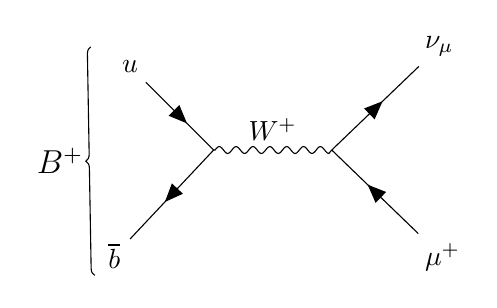
\begin{tikzpicture}
                    \begin{feynman}
                        \vertex (u) {\(\u\)}; 
                        \vertex [below right=of u] (v1);
                        \vertex [below left=of v1] (bbar) {\(\bbar\)}; 
                        \vertex [right=of v1] (v2);
                        \vertex [above right= of v2] (mu) {\(\nu_{\mu}\)};
                        \vertex [below right= of v2] (nu) {$\mu^{+}$};
                        \vertex [above left=0.25 and 0.5 of u] (u');
                        \vertex [below left=0.25 and 0.25 of bbar] (bbar');
                        \diagram*{
                            (u) -- [fermion] (v1) -- [fermion] (bbar),
                            (nu) -- [fermion] (v2) -- [fermion] (mu),
                            (v1) -- [photon,edge label={\(W^{+}\)}](v2),
                        };
                        \draw [decoration={brace}, decorate] (bbar') -- (u') node [pos=0.5, left] {\large $B^{+}$};
                    \end{feynman}    
                \end{tikzpicture}
            \end{center}
            \caption{A Feynman diagram of the decay \Bmunu, indicating the effect of Standard Model forces that facilitate this process.}%
            \label{fig:Bmunu}
        \end{figure}
        
        SM theory has also been used to mathematically predict and later experimentally confirm the existence of further ones.
        A complete explanation of the matter, mediator and resulting mathematical mechanisms of SM is not the focus of this thesis, and thus the scope is limited to how SM explains and predicts \Bmunu process.\\ 
        \begin{figure}[htpb]
            \centering
            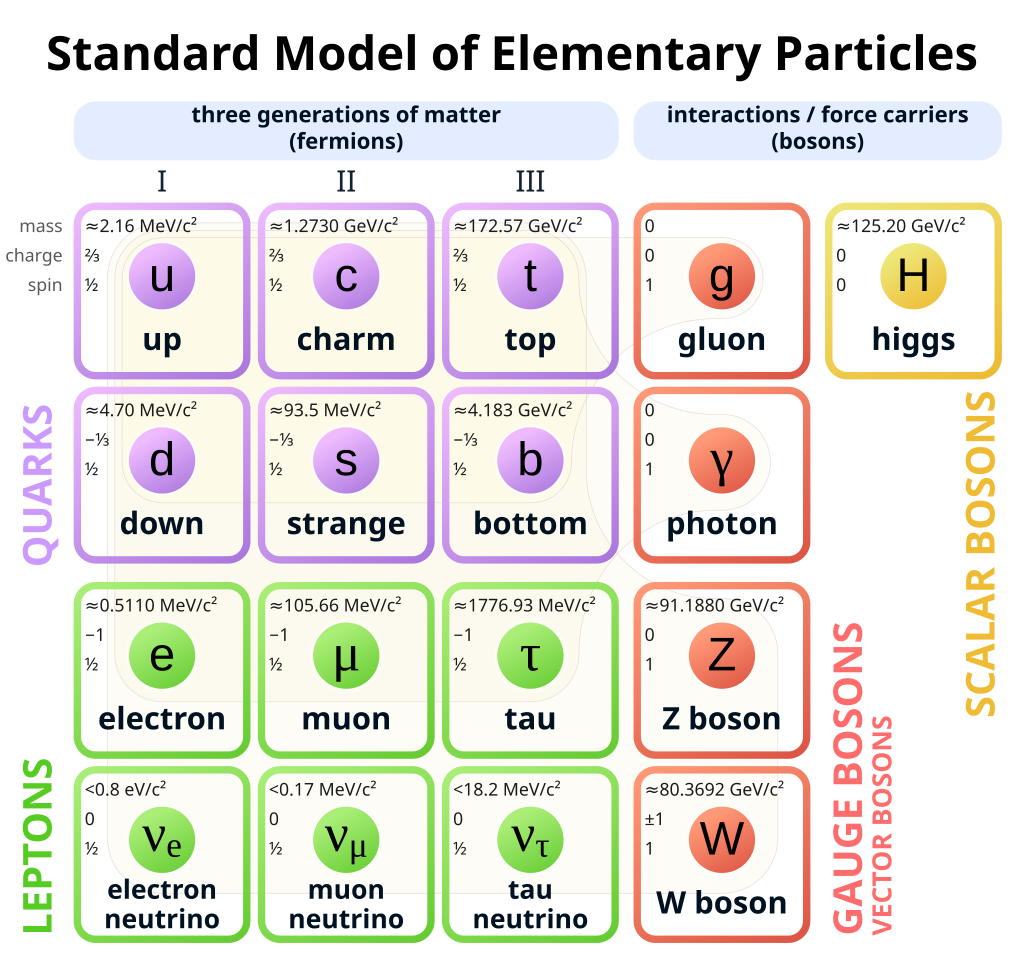
\includegraphics[width=0.62\textwidth]{./Intro/Figures/1024px-Standard_Model_of_Elementary_Particles.svg.png}
            \caption[The twelve fundamental fermions and five fundamental bosons of the Standard Model of Particle Physics. Each particle is uniquely defined by its mass, charge and intrinsic spin.]{The twelve fundamental fermions and five fundamental bosons of the Standard Model of Particle Physics\cite{pic:SM}. Each particle is uniquely defined by its mass, charge and intrinsic spin.} 
            \label{fig:SM}
        \end{figure}
        % Now we talk about pieces
        \subsection{Standard Model Particles and their Interactions}
            \subsubsection{Muons and neutrinos}
                The $\mu$ and $\nu_\mu$ in the final state of \Bmunu are a pair of matter particles referred to as \textit{leptons}.
                As seen in \Fig{fig:SM}, there are six leptons in SM, occurring in three generations of pairs between a neutral and a charged lepton.

\begin{center}
  $\bowtie$~$\bowtie$~$\bowtie$
\end{center}

  \chapter{The Belle II Experiment}
\label{chap:ch2}
\textit{In Chapter 2, blah blah blah} 
\begin{center}
  $\bowtie$~$\bowtie$~$\bowtie$
\end{center}
\section{The Belle II physics program}
    \subsection{Origins}
        Belle II is a high-energy physics experiment located at the SuperKEKB collider in Tsukuba, Japan.
        SuperKEKB is an asymmetric energy electron-positron collider, operating at a centre-of-mass energy equivalent to the \FourS resonance i.e. \sqrts=10.58\gev.
\section{Summary}
\begin{center}
  $\bowtie$~$\bowtie$~$\bowtie$
\end{center}

  %%etc
\end{mainmatter}

%%Appendices
\begin{appendices}
  \chapter{Appendix 1}
\section{Section 1}

  %%etc
\end{appendices}


%%Un-numbered back matter (bibliography, etc)
\begin{backmatter}
  
%\hypersetup{linkcolor=tab10Red}    %makes backref back to red    %not neccessary as in main.tex
%\bibliographystyle{h-physrev}
\bibliographystyle{JHEP_arXiv}
%\bibstyle{JHEP_arXiv}
\bibliography{main}

\end{backmatter}

\end{document}
